%! Tex program = pdflatex
 
\documentclass[UTF8]{ctexart}
\CTEXsetup[format={\Large\bfseries}]{section}
\usepackage{amsmath}
\usepackage{ctex}
\usepackage{array}
\usepackage{ulem}
\usepackage{graphicx}
\usepackage{geometry}
\usepackage{multirow}
\usepackage{subfig}
\usepackage{float}
\usepackage{multicol}
\usepackage{multirow}
\usepackage{indentfirst}
\usepackage{makecell}
\usepackage{listings, xcolor}
\lstdefinestyle{lfonts}{
  basicstyle   = \footnotesize\ttfamily,
  stringstyle  = \color{purple},
  keywordstyle = \color{blue!60!black}\bfseries,
  commentstyle = \color{olive}\scshape,
}
\lstdefinestyle{lnumbers}{
  numbers     = left,
  numberstyle = \tiny,
  numbersep   = 1em,
  firstnumber = 1,
  stepnumber  = 1,
}
\lstdefinestyle{llayout}{
  breaklines       = true,
  tabsize          = 2,
  columns          = flexible,
}
\lstdefinestyle{lgeometry}{
  xleftmargin      = 20pt,
  xrightmargin     = 0pt,
  frame            = tb,
  framesep         = \fboxsep,
  framexleftmargin = 20pt,
}
\lstdefinestyle{lgeneral}{
  style = lfonts,
  style = lnumbers,
  style = llayout,
  style = lgeometry,
}
\lstdefinestyle{python}{
  language = {Python},
  style    = lgeneral,
}
\geometry{papersize={21cm,29.7cm}}
\geometry{left=2.54cm,right=2.54cm,top=3.18cm,bottom=3.18cm}
\usepackage{fancyhdr}
\pagestyle{fancy}
\lhead{\today}
\chead{}
\rhead{2020011075}
\lfoot{清华大学}
\cfoot{\thepage}
\rfoot{系统工程导论}
\renewcommand{\headrulewidth}{0.4pt}
\renewcommand{\headwidth}{\textwidth}
\renewcommand{\footrulewidth}{0pt}
\usepackage{bm}

\begin{document}

\begin{center}
  \textbf{\LARGE{系统工程导论作业四——黑箱建模2}}\\
\end{center}
\begin{center}
  \large{彭程 2020011075}
\end{center}


\noindent \textbf{\zihao{-4}{1.试说明:病态线性回归问题中,显著性检验是否需要?}}\\

\noindent \textbf{结论:}

病态线性回归中需要显著性检验,且在自变量降维去线性之后进行检验。

\noindent \textbf{需要进行检验:}

显著性检验就是事先对总体(随机变量)的参数或总体分布形式做出一个假设,然后利用样本信息来判断这个假设(备择假设)是否合理,即判断总体的真实情况与原假设是否有显著性差异。在线性回归中体现为验证线性回归模型的有效性。病态线性回归问题也是利用样本信息来判断总体的参数,所以也需要显著性检验来确定总体分布形式假设是否合理,判断总体的真实情况与原假设是否有显著性差异,因此病态线性回归问题中也需要进行显著性检验。

\noindent \textbf{降维之后检验:}

病态回归问题中,由于自变量成线性相关或近似线性相关关系,所以自变量降维去线性之前,参数估计的误差可能会被严重放大,线性相关的变量的系数是不稳定的,因此即便是估计出来参数,意义也并不大,更没有必要进行显著性检验。 而在自变量降维去线性之后,线性回归误差较小,因此应该在此时进行显著性检验。\\


\noindent \textbf{\zihao{-4}{2.编程实现多元线性回归。}}\\

\noindent \textbf{\zihao{-4}{2.1 算法思路}}

\noindent 1.样本数据规范化,消除单位影响。

$$
\bar{x}_{i}(t)=\frac{x_{i}(t)-e\left(x_{i}\right)}{\sqrt{\delta^{2}\left(x_{i}\right)}} ~~\forall i, t
$$

其中,  $e\left(x_{i}\right)=\frac{1}{N} \sum_{t=1}^{N} x_{i}(t)$  为样本均值, $ \delta^{2}\left(x_{i}\right)=\frac{1}{N-1} \sum_{t=1}^{N} \left(x_{i}(t)-e\left(x_{i}\right)\right)^{2} $ 为样本方差
$$
\bar{y}(t)=\frac{y(t)-e(y)}{\sqrt{\delta^{2}(y)}} ~~\forall t
$$
\noindent 2.根据阈值确定最优维度m

对归一化的  $X X^{T}$  进行特征值分解, 得到 $ X X^{T}=Q \Lambda Q^{T} $。按照特征值从大到小选取特征向量, 直到相对逼近误差(末选取的特征值占特征值的比例)小于选取的阈值。\\

\noindent 3.求出降维后的矩阵。

将特征向量组成矩阵 $ Q_{m}=[q(1) q(2) \cdots q(m)] $,从而降维后的矩阵为$Z=Q_{m}^T X $。\\

\noindent 4.计算降维后的回归系数d,从而确定降维前的回归系数c,恢复得到归一化前的回归系数
$$
\begin{array}{c}
\hat{d}=\left(Z Z^{T}\right)^{-1} Z Y^{T} \\
\hat{c}=Q_{m} \hat{d}
\end{array}
$$

\noindent 5.进行显著性检验

对计算得到的回归系数进行显著性检验,注意其中n为降维之后的维度m:
$$
F=\frac{(N-n-1) E S S}{n R S S}
$$

\noindent 7.求取置信区间


给定显著性水平 $ \alpha $, 对某一  $\mathrm{x}_{0}$ , 相应的  $\mathrm{y}_{0} $ 将以 $ 1-\alpha$  的概率落在置信区间:
$$
\left(\hat{y}_{0}-Z_{\alpha / 2} S_{\delta}, \hat{y}_{0}+Z_{\alpha / 2} S_{\delta}\right)
$$

其中 $ Z_{\alpha / 2} $ 是标准正态分布上  $\alpha / 2 $ 百分位点的值, 剩余均方差  $S_{\delta}=\sqrt{\frac{R S S}{N-n-1}}$。\\

\noindent \textbf{\zihao{-4}{2.2 实验结果}}

\begin{figure}[H]
  \centering
  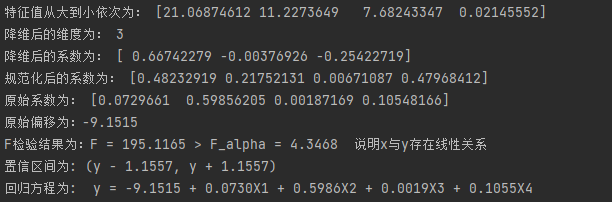
\includegraphics[scale=1.2]{实验结果.png}
\end{figure}

回归方程: $ y=-9.1515+0.0730 x_{1}+0.5986 x_{2}+0.0019 x_{3}+0.1055 x_{4} $\\

$ \mathrm{F}$  检验: $ \mathrm{F}=195.1165>4.3468$ , 因此  x, y  存在线性关系。\\

置信区间:  $[\mathrm{y}-1.1557, \mathrm{y}+1.1557] $\\

\noindent \textbf{\zihao{-4}{2.3 代码}}


\begin{lstlisting}[style = python]
import numpy as np
from scipy import stats

def linear_regression1(Y, X, alpha=0.05, error=0.01):
    """
    输入:n×N的矩阵X,1×N的矩阵Y
    输出:N×1的回归系数theta
    功能:实现Y=c^T*X+b的多元线性回归,自适应病态线性回归
    """
    n, N = X.shape

    # 数据规范化
    x_mean = np.mean(X, axis=1, keepdims=True)
    delta_x = np.sqrt(
        np.sum(np.multiply(X - np.mean(X, axis=1, keepdims=True), X - np.mean(X, axis=1, keepdims=True)), axis=1,
               keepdims=True) / (N - 1))
    X_normal = np.divide(X - x_mean, delta_x)
    y_mean = np.mean(Y)
    delta_y = np.sqrt(np.sum(np.multiply(Y - y_mean, Y - y_mean)) / (N - 1))
    Y_normal = (Y - y_mean) / delta_y

    # 根据阈值确定最优维度m
    eigenvalue, eigenvector = np.linalg.eig(np.dot(X_normal, X_normal.T))
    eigen_index = np.argsort(-eigenvalue)  # 返回排序的下标
    eigen_sum = np.sum(eigenvalue)
    for m in range(0, n):
        eigen_error = 0
        for i in range(0, m):
            eigen_error += eigenvalue[eigen_index[n - 1 - i]]
        eigen_error = eigen_error / eigen_sum
        if eigen_error > error:
            break
    m = n - m + 1  # 则前m项是要保留的

    # 计算降维后的回归系数d,从而确定降维前的回归系数c_n,恢复得到归一化前的回归系数c
    Q = eigenvector[:, eigen_index[0: m]]
    Z = Q.T.dot(X_normal)
    d = np.linalg.inv(Z.dot(Z.T)).dot(Z.dot(Y_normal.T))
    c_n = Q.dot(d)
    c = (c_n.T / np.squeeze(delta_x) * delta_y).T
    b = y_mean - np.sum(c * np.squeeze(x_mean))
    print("特征值从大到小依次为:", eigenvalue[eigen_index[:]])
    print("降维后的维度为:", m)
    print("降维后的系数为:", d)
    print("规范化后的系数为:", c_n)
    print("原始系数为:", c)
    print("原始偏移为:{:.4f}".format(b))

    # F检验操作
    Y_estimate = np.dot(c.T, X) + b
    ESS = np.dot((Y_estimate - y_mean), (Y_estimate - y_mean).T)
    RSS = np.dot((Y - Y_estimate), (Y - Y_estimate).T)
    F = ((N - m - 1) * ESS) / (m * RSS)  # ESS自由度为(N-m-1),RSS自由度为m
    F_alpha = stats.f.isf(alpha, m, N - m - 1)
    if F > F_alpha:
        print("F检验结果为:F = {:.4f} > F_alpha = {:.4f}".format(F, F_alpha), " 说明x与y存在线性关系")
    elif F <= F_alpha:
        print("F检验结果为:")
        print("F-value = {} <= F_alpha = {}".format(F, F_alpha))
        print("x与y不存在线性关系")
        return 0

    # 置信区间
    S_delta = np.sqrt(RSS / (N - m - 1))
    Z_alpha_div2 = stats.norm.isf(alpha / 2, 0, 1)
    interval = Z_alpha_div2 * S_delta
    print("置信区间为: (y - {:.4f}, y + {:.4f})".format(interval, interval))

    # 打印回归方程
    equation = "y = %.4f" % b
    for i in range(n):
        equation += " + %.4fX%d" % (c[i], i + 1)
    print("回归方程为: ", equation)

    return


if __name__ == '__main__':
    f = open('data.txt', 'r', encoding='utf-8')
    # raw_data = np.array([list(map(float, i[:-1].split(' '))) for i in f.readlines()[1:]])
    raw_data = np.array([i[:-1].split(' ') for i in f.readlines()[1:]], dtype=float)
    x = raw_data[:, 1: 5]
    y = raw_data[:, -1]
    linear_regression1(y.T, x.T, 0.05, 0.01)

\end{lstlisting}      


\end{document}